\documentclass[12pt, a4paper]{article}

% ── Paquetes ──
\usepackage[utf8]{inputenc}
\usepackage[T1]{fontenc}
\usepackage[spanish]{babel}
\usepackage{geometry}
\usepackage{setspace}
\usepackage{parskip}
\usepackage{hyperref}
\usepackage{enumitem}
\usepackage{titlesec}
\usepackage{fancyhdr}
\usepackage{xcolor}
\usepackage{graphicx}
\usepackage{tikz}
\usepackage{amsmath}
\usepackage{amssymb}
\usepackage{booktabs}
\usepackage{float}
\usepackage{caption}

\geometry{margin=2.5cm}
\onehalfspacing
\graphicspath{{graficos/}{./}}

% ── Colores ──
\definecolor{accent}{RGB}{0, 90, 130}
\definecolor{ucblue}{RGB}{0, 75, 135}
\definecolor{ucgold}{RGB}{198, 166, 80}

% ── Formato de secciones ──
\titleformat{\section}{\large\bfseries\color{accent}}{}{0em}{}[\vspace{-0.5em}\color{accent}\rule{\textwidth}{0.4pt}]
\titleformat{\subsection}{\normalsize\bfseries\color{accent!80!black}}{}{0em}{}

% ── Encabezado ──
\pagestyle{fancy}
\fancyhf{}
\fancyhead[L]{\small\textit{Control 1 -- Semanas 01 a 04}}
\fancyhead[R]{\small\textit{Recuperación de Información}}
\fancyfoot[C]{\thepage}
\renewcommand{\headrulewidth}{0.4pt}

\hypersetup{
    colorlinks=true,
    linkcolor=accent,
    urlcolor=accent!70!black,
    citecolor=accent,
    pdftitle={Control 1 - INF3841 Recuperación de Información},
    pdfauthor={Armando Arredondo Valle},
    pdfsubject={Recuperación de Información}
}

% celda vacía en las matrices de resultado
\newcommand{\vacia}{\phantom{0000}}

% ══════════════════════════════════════════════════════════════════════
\begin{document}

% ── Portada ──
\begin{titlepage}
    \begin{tikzpicture}[remember picture, overlay]
        \fill[ucblue] (current page.north west) rectangle ([yshift=-4cm]current page.north east);
        \fill[ucgold] ([yshift=-4cm]current page.north west) rectangle ([yshift=-4.15cm]current page.north east);
        \fill[ucblue] (current page.south west) rectangle ([yshift=2cm]current page.south east);
        \fill[ucgold] ([yshift=2cm]current page.south west) rectangle ([yshift=2.15cm]current page.south east);
    \end{tikzpicture}

    \centering
    \vspace*{1.2cm}

    
\includegraphics[width=5.5cm]{Logo.png}

    \vspace{1.5cm}

    {\color{ucblue}\rule{0.6\textwidth}{0.8pt}}

    \vspace{0.8cm}

    {\LARGE\bfseries\color{ucblue} Control 1}

    \vspace{1.2cm}

    {\Large\color{black} Procesamiento de imágenes, detección de bordes,\\[0.2em]
    descriptores globales de gris y color, y audio digital}

    \vspace{0.8cm}

    {\color{ucblue}\rule{0.6\textwidth}{0.8pt}}

    \vspace{1.5cm}

    {\large\bfseries Armando Arredondo Valle}

    \vspace{0.6cm}

    {\normalsize Magíster en Inteligencia Artificial\\[0.2em]
    INF3841 Recuperación de Información\\[0.2em]
    Profesor: Juan Manuel Barrios\\[0.5em]
    Pontificia Universidad Católica de Chile}

    \vfill

    {\normalsize 23 de agosto de 2026}

    \vspace{1.5cm}
\end{titlepage}

% ══════════════════════════════════════════════════════════════════════
\section{Semana 01}

\subsection{a) i. Convolución $A * K$}

Las celdas vacías son las posiciones donde la máscara de $3 \times 3$ no queda completamente contenida en la imagen.

\[
A * K =
\begin{bmatrix}
\vacia & \vacia & \vacia & \vacia & \vacia \\
\vacia & 1200 & -900 & 450 & \vacia \\
\vacia & -900 & 900 & -900 & \vacia \\
\vacia & 450 & -900 & 1200 & \vacia \\
\vacia & \vacia & \vacia & \vacia & \vacia
\end{bmatrix}
\]

\subsection{a) ii. Umbral $U_t$ con $t = 1000$}

\[
U_{1000}(A * K) =
\begin{bmatrix}
\vacia & \vacia & \vacia & \vacia & \vacia \\
\vacia & 255 & 0 & 0 & \vacia \\
\vacia & 0 & 0 & 0 & \vacia \\
\vacia & 0 & 0 & 255 & \vacia \\
\vacia & \vacia & \vacia & \vacia & \vacia
\end{bmatrix}
\]

\subsection{a) iii. Filtro de mediana de $3 \times 3$ sobre $A$}

\[
\text{mediana}_{3\times3}(A) =
\begin{bmatrix}
\vacia & \vacia & \vacia & \vacia & \vacia \\
\vacia & 200 & 50 & 50 & \vacia \\
\vacia & 50 & 50 & 50 & \vacia \\
\vacia & 50 & 50 & 200 & \vacia \\
\vacia & \vacia & \vacia & \vacia & \vacia
\end{bmatrix}
\]

\subsection{b) i. $B_x = B * S_x$}

Gradiente calculado por correlación con la máscara de Sobel, igual que \texttt{cv2.Sobel()}.

\[
B_x =
\begin{bmatrix}
\vacia & \vacia & \vacia & \vacia & \vacia & \vacia & \vacia \\
\vacia & -128 & -384 & -384 & -128 & 0 & \vacia \\
\vacia & -384 & -384 & -128 & 0 & -127 & \vacia \\
\vacia & -384 & -128 & 0 & -127 & -381 & \vacia \\
\vacia & -128 & 0 & -127 & -381 & -381 & \vacia \\
\vacia & 0 & -127 & -381 & -381 & -127 & \vacia \\
\vacia & \vacia & \vacia & \vacia & \vacia & \vacia & \vacia
\end{bmatrix}
\]

\subsection{b) ii. $B_y = B * S_y$}

$B$ es simétrica respecto de su transpuesta y $S_y = S_x^{\mathsf{T}}$, por lo que $B_y = B_x$.

\[
B_y =
\begin{bmatrix}
\vacia & \vacia & \vacia & \vacia & \vacia & \vacia & \vacia \\
\vacia & -128 & -384 & -384 & -128 & 0 & \vacia \\
\vacia & -384 & -384 & -128 & 0 & -127 & \vacia \\
\vacia & -384 & -128 & 0 & -127 & -381 & \vacia \\
\vacia & -128 & 0 & -127 & -381 & -381 & \vacia \\
\vacia & 0 & -127 & -381 & -381 & -127 & \vacia \\
\vacia & \vacia & \vacia & \vacia & \vacia & \vacia & \vacia
\end{bmatrix}
\]

\subsection{b) iii. Magnitud del gradiente}

\[
\sqrt{B_x^2 + B_y^2} =
\begin{bmatrix}
\vacia & \vacia & \vacia & \vacia & \vacia & \vacia & \vacia \\
\vacia & 181{,}0 & 543{,}1 & 543{,}1 & 181{,}0 & 0{,}0 & \vacia \\
\vacia & 543{,}1 & 543{,}1 & 181{,}0 & 0{,}0 & 179{,}6 & \vacia \\
\vacia & 543{,}1 & 181{,}0 & 0{,}0 & 179{,}6 & 538{,}8 & \vacia \\
\vacia & 181{,}0 & 0{,}0 & 179{,}6 & 538{,}8 & 538{,}8 & \vacia \\
\vacia & 0{,}0 & 179{,}6 & 538{,}8 & 538{,}8 & 179{,}6 & \vacia \\
\vacia & \vacia & \vacia & \vacia & \vacia & \vacia & \vacia
\end{bmatrix}
\]

\subsection{b) iv. Ángulo del gradiente en $[-180^\circ, 180^\circ]$}

El ángulo no está definido donde la magnitud del gradiente es $0$; esas celdas se dejan vacías, igual que el borde.

\[
\operatorname{arctan2}(B_y, B_x) =
\begin{bmatrix}
\vacia & \vacia & \vacia & \vacia & \vacia & \vacia & \vacia \\
\vacia & -135 & -135 & -135 & -135 & \vacia & \vacia \\
\vacia & -135 & -135 & -135 & \vacia & -135 & \vacia \\
\vacia & -135 & -135 & \vacia & -135 & -135 & \vacia \\
\vacia & -135 & \vacia & -135 & -135 & -135 & \vacia \\
\vacia & \vacia & -135 & -135 & -135 & -135 & \vacia \\
\vacia & \vacia & \vacia & \vacia & \vacia & \vacia & \vacia
\end{bmatrix}
\]

Todos los ángulos definidos valen $-135^\circ$: $B$ decrece de $255$ en la esquina superior izquierda a $0$ en la inferior derecha, y el gradiente apunta hacia donde la intensidad crece.

% ══════════════════════════════════════════════════════════════════════
\section{Semana 02}

\subsection{i. Histograma global de 256 bins}

Cada bin representa un tono de gris; el bin $k$ cuenta los pixeles de valor $k-1$. Los 253 bins no listados tienen altura 0.

\begin{table}[H]
\centering
\caption{Bins distintos de cero del histograma global de $I$.}
\begin{tabular}{clrr}
\toprule
\textbf{Bin} & \textbf{Tono que representa} & \textbf{Pixeles} & \textbf{Altura} \\
\midrule
1 & 0 & 22 & 0,3438 \\
128 & 127 & 18 & 0,2812 \\
256 & 255 & 24 & 0,3750 \\
\midrule
\multicolumn{2}{l}{\textbf{Total}} & \textbf{64} & \textbf{1,0000} \\
\bottomrule
\end{tabular}
\end{table}

\begin{figure}[H]
\centering
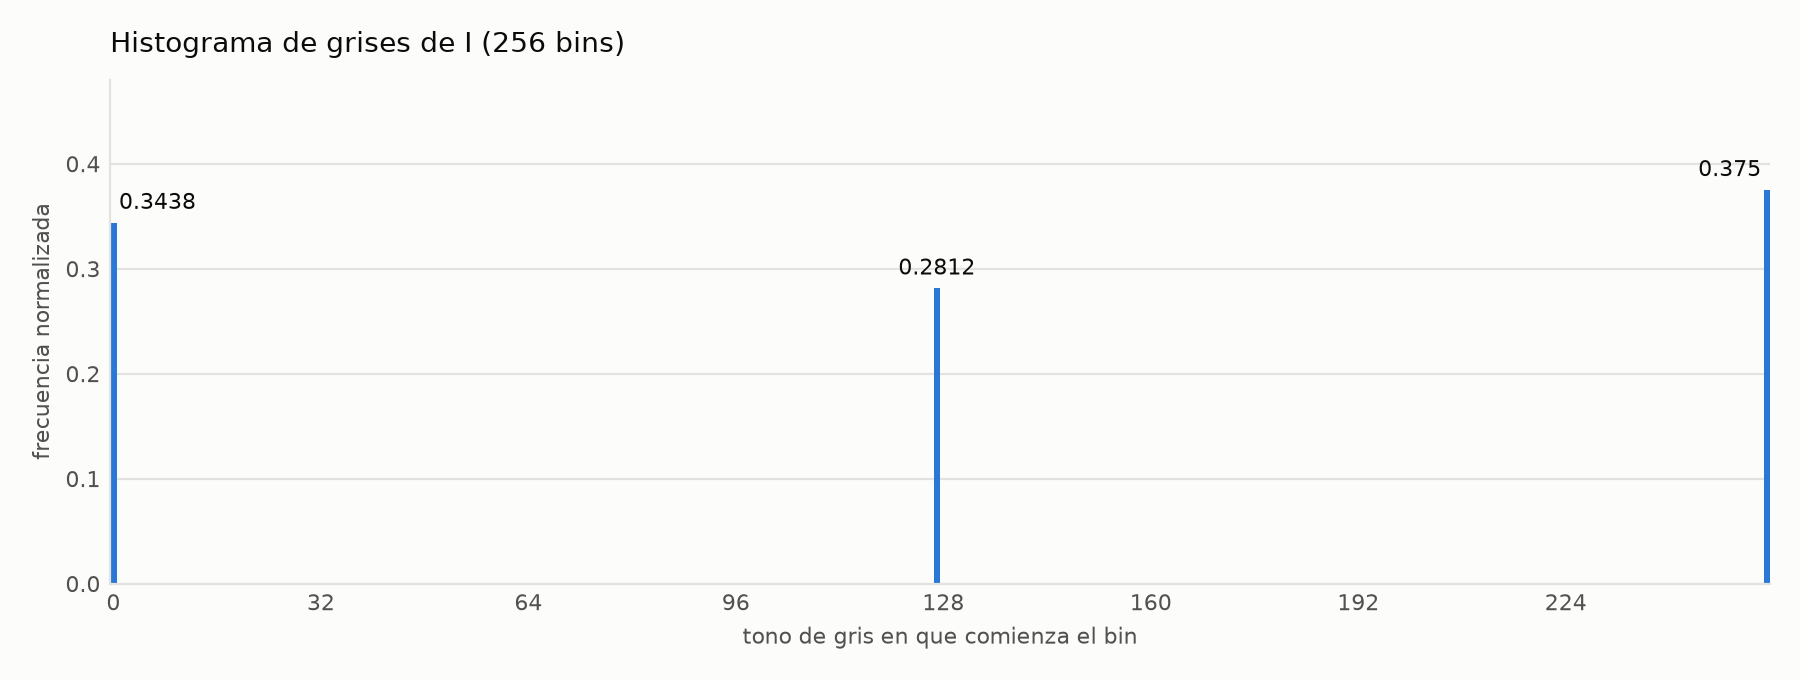
\includegraphics[width=\textwidth]{semana02-i-histograma-global.png}
\caption{Histograma de grises de $I$ con 256 bins normalizados.}
\end{figure}

\subsection{ii. Histograma de 256 bins en $2 \times 2$ zonas}

Cada zona cubre $4 \times 4 = 16$ pixeles y su histograma se normaliza por separado. El descriptor completo es la concatenación de los cuatro histogramas: $4 \times 256 = 1024$ dimensiones.

\begin{table}[H]
\centering
\caption{Bins distintos de cero de cada zona de $I$.}
\begin{tabular}{llrr}
\toprule
\textbf{Zona} & \textbf{Bin (tono)} & \textbf{Pixeles} & \textbf{Altura} \\
\midrule
Fila 1, columna 1 & 1 (0) & 6 & 0,3750 \\
                  & 128 (127) & 10 & 0,6250 \\
\midrule
Fila 1, columna 2 & 1 (0) & 8 & 0,5000 \\
                  & 256 (255) & 8 & 0,5000 \\
\midrule
Fila 2, columna 1 & 1 (0) & 8 & 0,5000 \\
                  & 256 (255) & 8 & 0,5000 \\
\midrule
Fila 2, columna 2 & 128 (127) & 8 & 0,5000 \\
                  & 256 (255) & 8 & 0,5000 \\
\bottomrule
\end{tabular}
\end{table}

\begin{figure}[H]
\centering
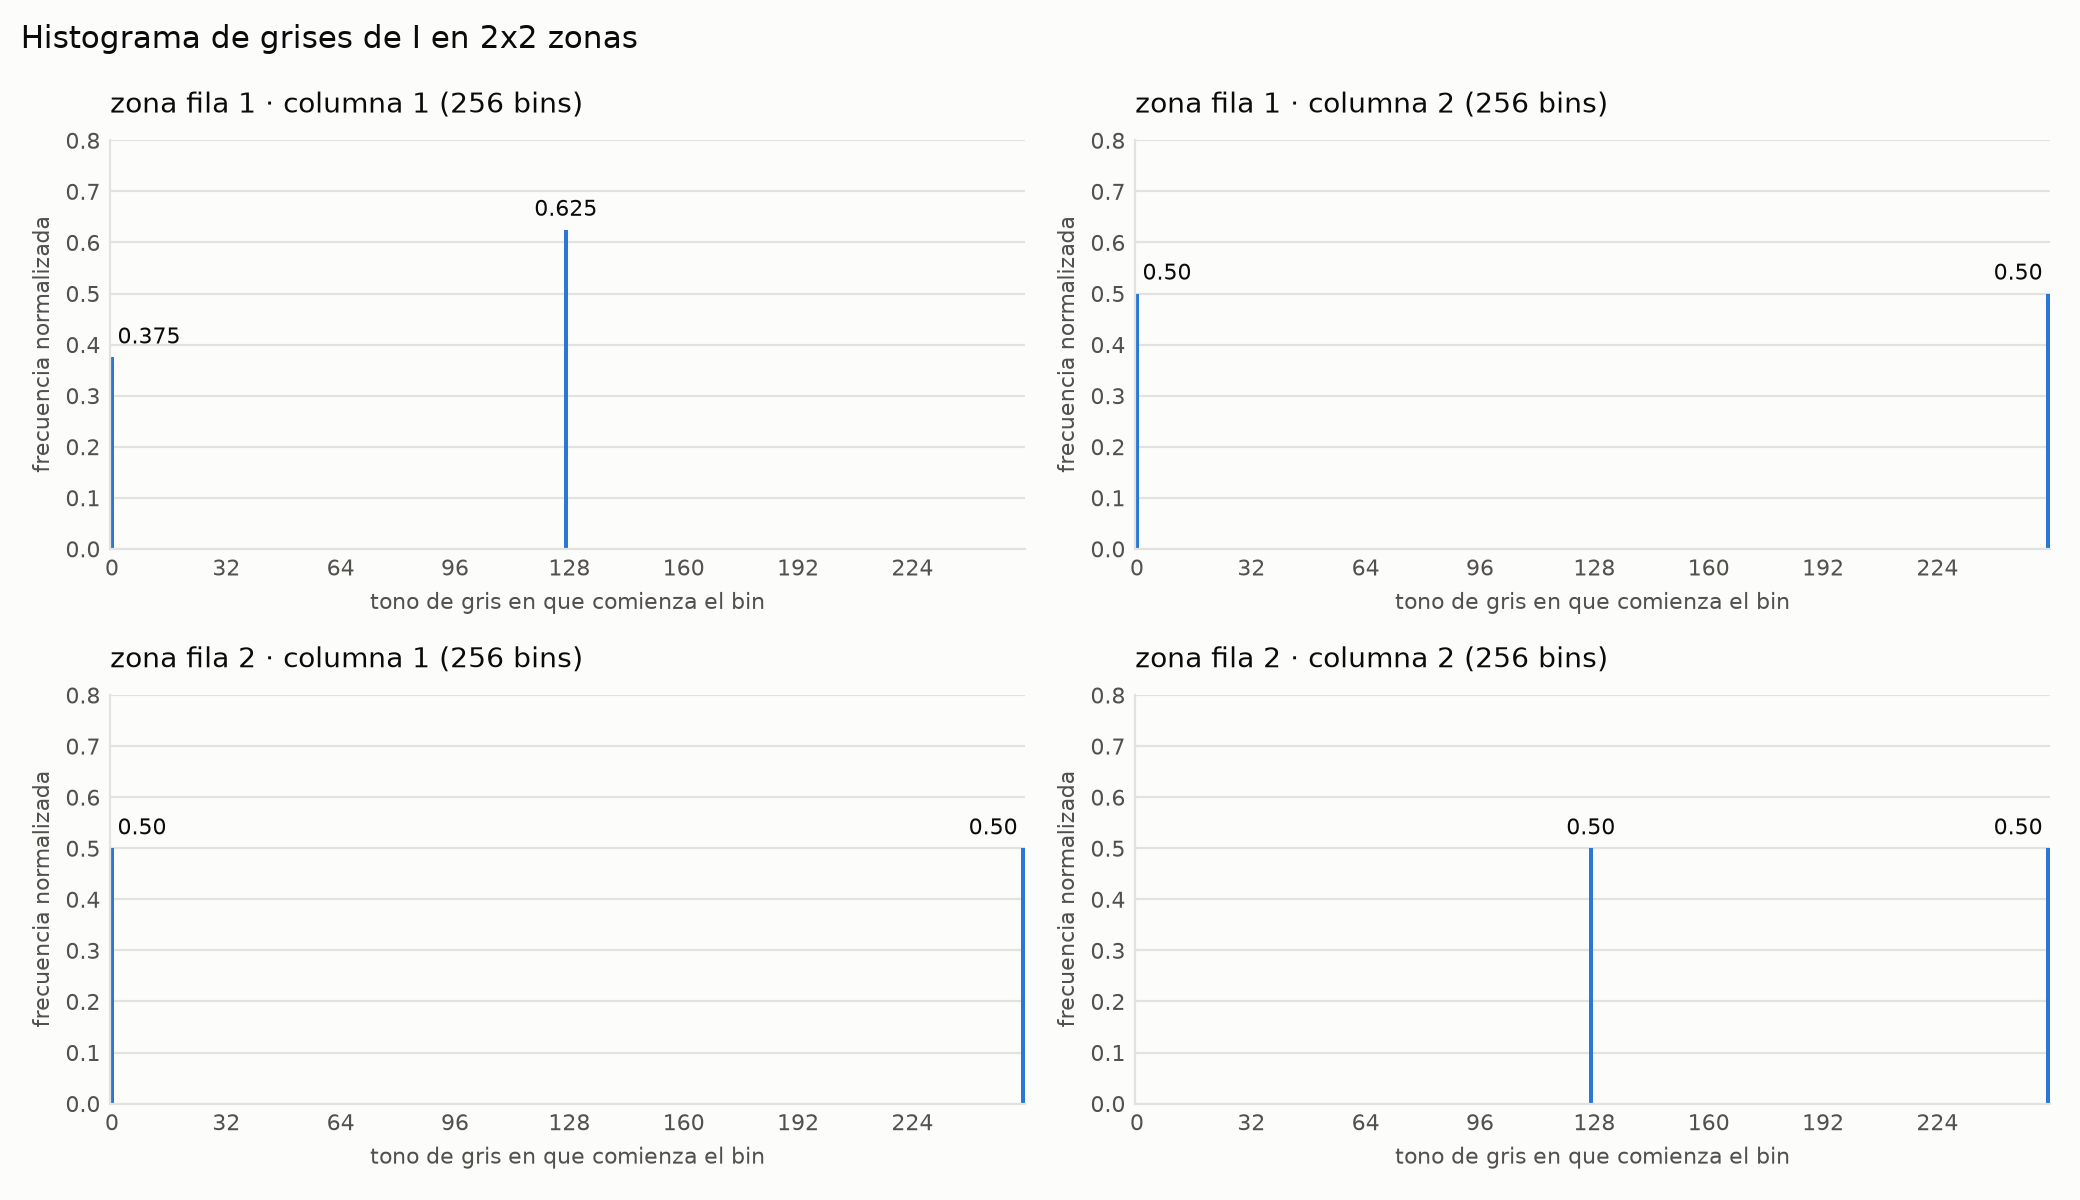
\includegraphics[width=\textwidth]{semana02-ii-histograma-zonas.png}
\caption{Histogramas de 256 bins de cada zona de $I$, con la misma escala vertical.}
\end{figure}

\subsection{iii. HOG en $2 \times 2$ zonas}

Gradiente por Sobel calculado dentro de cada zona (división estricta), pixeles con magnitud mayor o igual a 200, ángulos llevados al rango $(-90^\circ, 90^\circ]$ y acumulados en 9 bins de $20^\circ$ cada uno.

\begin{table}[H]
\centering
\caption{Ángulos de los pixeles de borde de cada zona y bin en que se acumulan.}
\begin{tabular}{llcl}
\toprule
\textbf{Zona} & \textbf{Ángulos de borde} & \textbf{Pixeles} & \textbf{Bin resultante} \\
\midrule
Fila 1, columna 1 & $-45^\circ$ (tres veces) & 3 & bin 3: $(-50^\circ, -30^\circ]$, altura 1,00 \\
Fila 1, columna 2 & ninguno & 0 & histograma nulo \\
Fila 2, columna 1 & $90^\circ$ (cuatro veces) & 4 & bin 9: $(70^\circ, 90^\circ]$, altura 1,00 \\
Fila 2, columna 2 & $0^\circ$ (cuatro veces) & 4 & bin 5: $(-10^\circ, 10^\circ]$, altura 1,00 \\
\bottomrule
\end{tabular}
\end{table}

\begin{figure}[H]
\centering
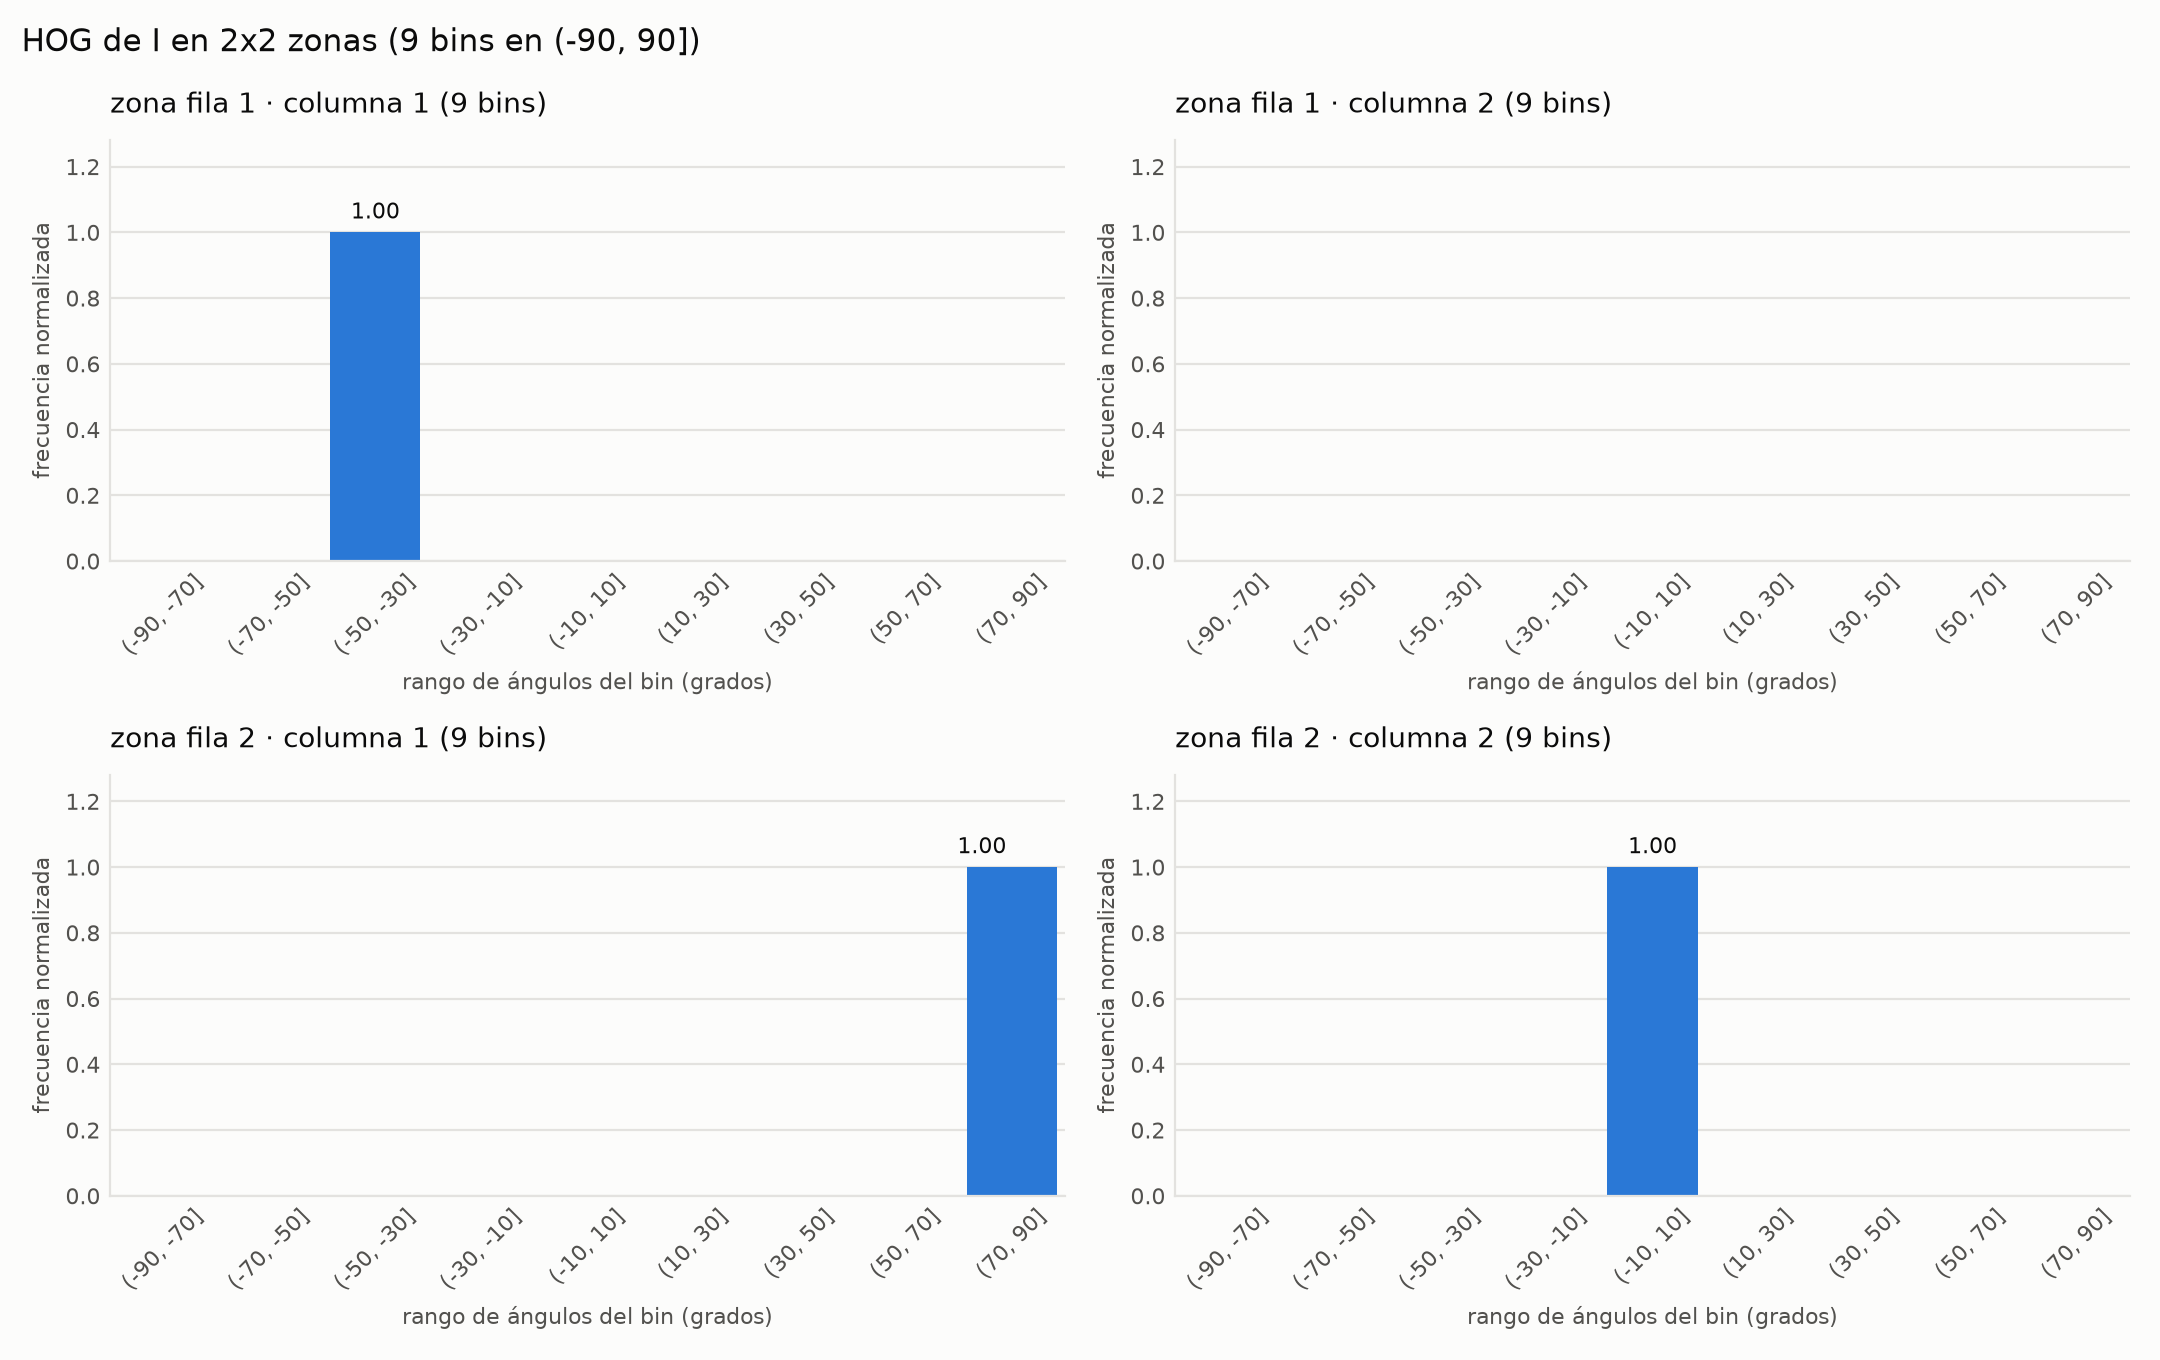
\includegraphics[width=\textwidth]{semana02-iii-hog-zonas.png}
\caption{HOG de cada zona de $I$: 9 bins que cubren el rango $(-90^\circ, 90^\circ]$.}
\end{figure}

En la zona de la fila 1, columna 2 (tablero de ajedrez de periodo 2) las respuestas de Sobel se cancelan y la magnitud del gradiente es 0 en los cuatro pixeles interiores, por lo que ningún pixel alcanza el umbral y el histograma queda nulo.

% ══════════════════════════════════════════════════════════════════════
\section{Semana 03}

\subsection{a) i. Histograma global por canal 4+4+4}

Cada canal se divide en 4 bins regulares sobre $[0, 256)$ y se normaliza por separado. La imagen $D$ tiene $9 \times 6 = 54$ pixeles: 8 azules $(0, 50, 160)$, 19 blancos $(255, 255, 255)$ y 27 rojos $(218, 41, 28)$.

\begin{table}[H]
\centering
\caption{Bins distintos de cero de cada canal de $D$.}
\begin{tabular}{cclrr}
\toprule
\textbf{Canal} & \textbf{Bin} & \textbf{Rango que representa} & \textbf{Pixeles} & \textbf{Altura} \\
\midrule
R & 1 & $[0, 63]$ & 8 & 0,1481 \\
  & 4 & $[192, 255]$ & 46 & 0,8519 \\
\midrule
G & 1 & $[0, 63]$ & 35 & 0,6481 \\
  & 4 & $[192, 255]$ & 19 & 0,3519 \\
\midrule
B & 1 & $[0, 63]$ & 27 & 0,5000 \\
  & 3 & $[128, 191]$ & 8 & 0,1481 \\
  & 4 & $[192, 255]$ & 19 & 0,3519 \\
\bottomrule
\end{tabular}
\end{table}

\begin{figure}[H]
\centering
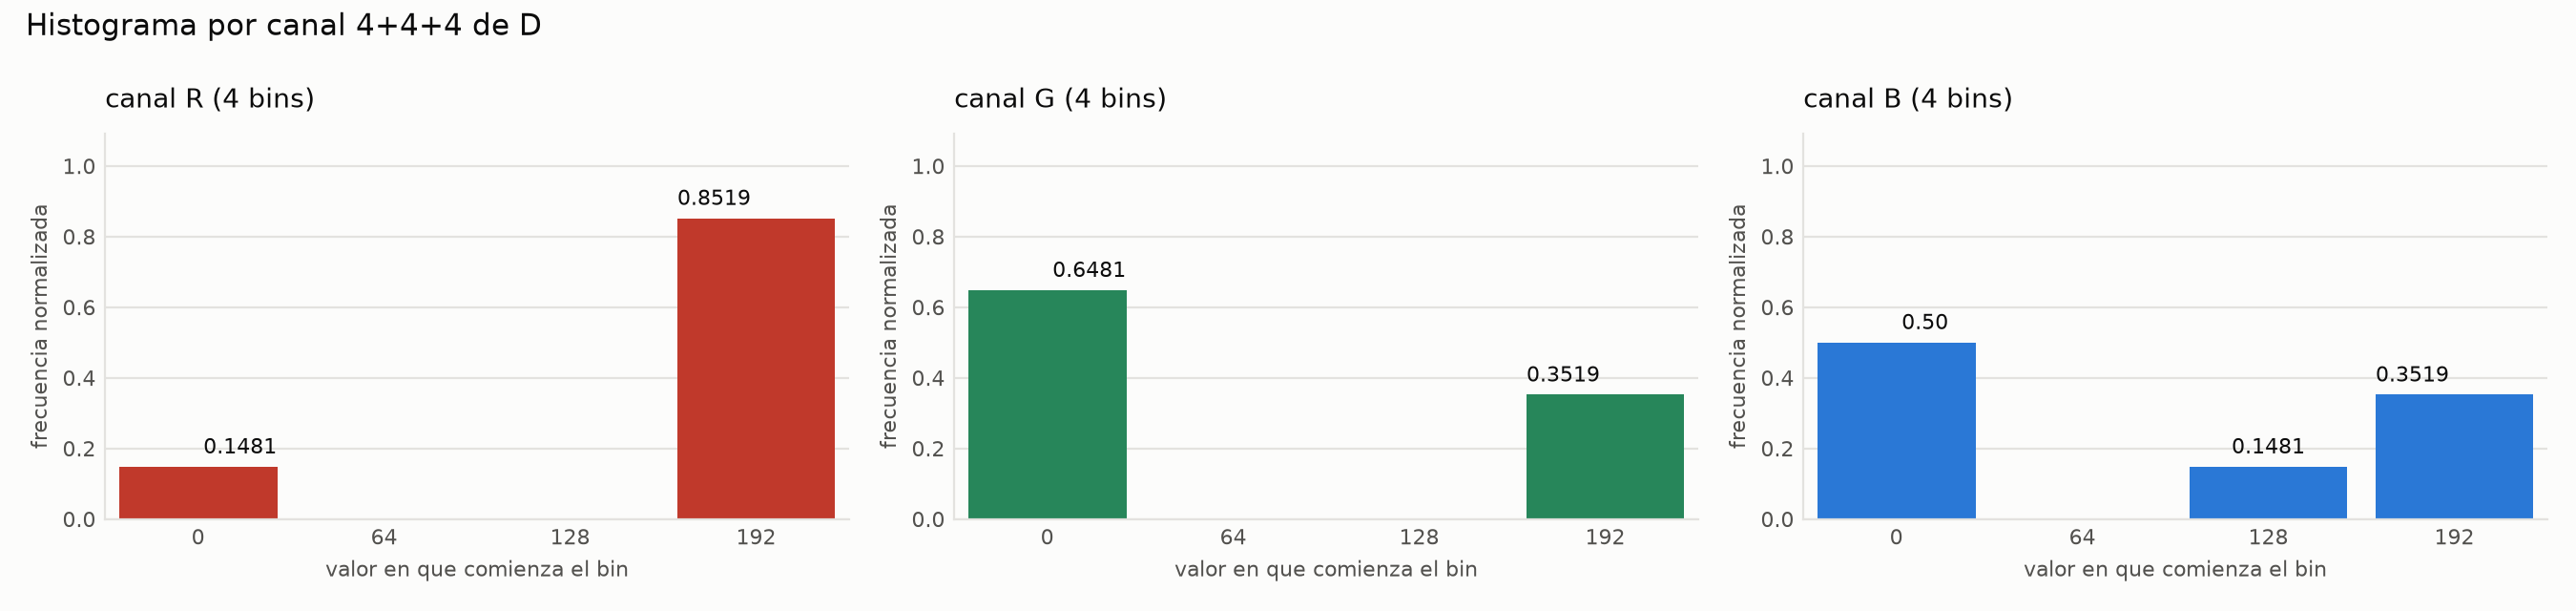
\includegraphics[width=\textwidth]{semana03-i-histograma-canales.png}
\caption{Histogramas de 4 bins de cada canal de $D$, normalizados por separado.}
\end{figure}

\subsection{a) ii. Histograma 3D RGB $4 \times 4 \times 4$}

El cubo RGB se divide en $4^3 = 64$ bins. Como $D$ tiene sólo tres colores distintos, sólo 3 bins son distintos de cero y cada uno concentra todos los pixeles de un color.

\begin{table}[H]
\centering
\caption{Bins distintos de cero del histograma 3D de $D$.}
\begin{tabular}{lccc r}
\toprule
\textbf{Bin $(R, G, B)$} & \textbf{Rango R} & \textbf{Rango G} & \textbf{Rango B} & \textbf{Altura} \\
\midrule
$(4, 1, 1)$ & $[192, 255]$ & $[0, 63]$ & $[0, 63]$ & 0,5000 \\
$(4, 4, 4)$ & $[192, 255]$ & $[192, 255]$ & $[192, 255]$ & 0,3519 \\
$(1, 1, 3)$ & $[0, 63]$ & $[0, 63]$ & $[128, 191]$ & 0,1481 \\
\midrule
\multicolumn{4}{l}{\textbf{Total}} & \textbf{1,0000} \\
\bottomrule
\end{tabular}
\end{table}

Los 61 bins restantes tienen altura 0.

\subsection{b) i. Matriz de costos}

Ground-distance: distancia euclidiana en CIE LAB (D65).

\begin{table}[H]
\centering
\caption{Colores de ambos histogramas convertidos a CIE LAB.}
\begin{tabular}{llrrr}
\toprule
\textbf{Histograma} & \textbf{Color RGB} & \textbf{$L$} & \textbf{$a$} & \textbf{$b$} \\
\midrule
1, bin 1 & $(85, 137, 184)$ & 55,33 & $-3{,}78$ & $-29{,}84$ \\
1, bin 2 & $(211, 56, 69)$ & 48,31 & 60,36 & 29,50 \\
1, bin 3 & $(19, 34, 103)$ & 16,76 & 21,45 & $-41{,}97$ \\
\midrule
2, bin 1 & $(233, 47, 36)$ & 51,17 & 68,20 & 51,72 \\
2, bin 2 & $(15, 42, 162)$ & 24,82 & 38,84 & $-66{,}05$ \\
2, bin 3 & $(140, 211, 247)$ & 81,12 & $-13{,}00$ & $-24{,}50$ \\
\bottomrule
\end{tabular}
\end{table}

Las filas son los bins del histograma 1 y las columnas los del histograma 2:

\[
K =
\begin{bmatrix}
108{,}86 & 63{,}71 & 27{,}90 \\
23{,}74 & 100{,}72 & 96{,}82 \\
110{,}21 & 30{,}77 & 75{,}06
\end{bmatrix}
\]

\subsection{b) ii. Matriz de flujos}

La EMD es el costo \emph{mínimo}, así que el flujo debe ser el de menor costo total. Se construye llenando primero las celdas más baratas y moviendo en cada una toda la masa posible.

\[
F =
\begin{bmatrix}
0{,}00 & 0{,}30 & 0{,}25 \\
0{,}25 & 0{,}05 & 0{,}00 \\
0{,}00 & 0{,}15 & 0{,}00
\end{bmatrix}
\]

Es un flujo válido: no tiene valores negativos, las filas suman $0{,}55$, $0{,}30$ y $0{,}15$ (los pesos del histograma 1) y las columnas suman $0{,}25$, $0{,}50$ y $0{,}25$ (los del histograma 2).

\subsection{b) iii. EMD}

\[
\mathrm{EMD} = \sum_{i}\sum_{j} K_{ij} \, F_{ij} = 41{,}6742 \approx 41{,}67
\]

Detalle del cálculo, celda por celda:

\[
\begin{aligned}
\mathrm{EMD} =\ & 0{,}30 \times 63{,}71 + 0{,}25 \times 27{,}90 \\
+\ & 0{,}25 \times 23{,}74 + 0{,}05 \times 100{,}72 \\
+\ & 0{,}15 \times 30{,}77 \;=\; 41{,}6742
\end{aligned}
\]

Como ambos histogramas están normalizados, el flujo total es 1 y el valor coincide con la versión normalizada $\sum K_{ij} F_{ij} / \sum F_{ij}$.

% ══════════════════════════════════════════════════════════════════════
\section{Semana 04}

La canción dura 1 minuto 37 segundos $= 97$ segundos. El enunciado no indica la cantidad de canales, por lo que se asume \textbf{un canal (mono)}; con estéreo todos los tamaños se duplican.

En PCM sin comprimir el tamaño es
\[
\text{bytes} = \text{duración} \times \text{sample rate} \times \frac{\text{bits por muestra}}{8} \times \text{canales}
\]
y la frecuencia máxima representable es la de Nyquist, la mitad del sample rate.

\begin{table}[H]
\centering
\caption{Resumen de los tres archivos.}
\begin{tabular}{llrrrr}
\toprule
\textbf{Archivo} & \textbf{Formato} & \textbf{Sample rate} & \textbf{Tamaño (bytes)} & \textbf{Nyquist} & \textbf{Frec. máx.} \\
\midrule
A.raw & s16le (16 bits) & 44.100 Hz & $8\,555\,400$ & 22.050 Hz & 22.050 Hz \\
B.raw & 32f (32 bits) & 8.192 Hz & $3\,178\,496$ & 4.096 Hz & 4.096 Hz \\
C.raw & s16le (16 bits) & 44.100 Hz & $8\,555\,400$ & 22.050 Hz & 4.096 Hz \\
\bottomrule
\end{tabular}
\end{table}

\subsection{i. A.raw (s16le, 44.100 Hz)}

$97 \times 44100 \times 2 \times 1 = 8\,555\,400$ bytes. Frecuencia máxima audible: $44100 / 2 = 22.050$ Hz.

\textbf{Peor calidad que el original:} bajar de 96 kHz a 44,1 kHz elimina todo lo que estaba sobre los 22.050 Hz y pasar de 64 bits a 16 reduce el rango dinámico. En la práctica la diferencia es casi inaudible, porque el oído humano no llega a 22 kHz.

\subsection{ii. B.raw (32f, 8.192 Hz)}

$97 \times 8192 \times 4 \times 1 = 3\,178\,496$ bytes. Frecuencia máxima audible: $8192 / 2 = 4.096$ Hz.

\textbf{Peor que A.raw:} aunque cada muestra tiene más bits (32f contra 16), el sample rate corta todo sobre 4.096 Hz, que es una pérdida claramente audible; la mayor profundidad no compensa la pérdida de ancho de banda.

\subsection{iii. C.raw (s16le, 44.100 Hz, convertido desde B.raw)}

$97 \times 44100 \times 2 \times 1 = 8\,555\,400$ bytes, el mismo tamaño que A.raw. La frecuencia máxima del \emph{formato} vuelve a ser 22.050 Hz, pero el \emph{contenido} sigue limitado a \textbf{4.096 Hz}.

\textbf{Peor que A.raw:} remuestrear hacia arriba no recupera las frecuencias que B.raw ya había perdido. C.raw ocupa el mismo espacio que A.raw y suena igual que B.raw.

\end{document}
